\documentclass[10pt]{article}
\usepackage[polish]{babel}
\usepackage[utf8]{inputenc}
\usepackage[T1]{fontenc}
\usepackage{amsmath}
\usepackage{amsfonts}
\usepackage{amssymb}
\usepackage[version=4]{mhchem}
\usepackage{stmaryrd}
\usepackage{graphicx}
\usepackage[export]{adjustbox}
\graphicspath{ {./images/} }

%New command to display footnote whose markers will always be hidden
\let\svthefootnote\thefootnote
\newcommand\blfootnotetext[1]{%
  \let\thefootnote\relax\footnote{#1}%
  \addtocounter{footnote}{-1}%
  \let\thefootnote\svthefootnote%
}

%Overriding the \footnotetext command to hide the marker if its value is `0`
\let\svfootnotetext\footnotetext
\renewcommand\footnotetext[2][?]{%
  \if\relax#1\relax%
    \ifnum\value{footnote}=0\blfootnotetext{#2}\else\svfootnotetext{#2}\fi%
  \else%
    \if?#1\ifnum\value{footnote}=0\blfootnotetext{#2}\else\svfootnotetext{#2}\fi%
    \else\svfootnotetext[#1]{#2}\fi%
  \fi
}

\newcommand\Varangle{\mathop{{<\!\!\!\!\!\text{\small)}}\:}\nolimits}

\begin{document}
\section*{CENTRALNA \\
 KOMISJA \\
 EGZAMINACYJNA}
\begin{center}
\begin{tabular}{|l|l|}
\hline
Rodzaj dokumentu: & \begin{tabular}{l}
Zasady oceniania rozwiązań \\
zadań \\
\end{tabular} \\
\hline
Egzamin: & Egzamin maturalny \\
\hline
Przedmiot: & Matematyka \\
\hline
Poziom: & \begin{tabular}{l}
EMAP-P0-100-2205 (wersje arkusza: A i B), \\
EMAP-P0-200-2205, EMAP-P0-300-2205, \\
\hline
Formy arkusza: \\
\hline
\end{tabular} \\
\hline
EMAP-P0-400-2205, EMAP-P0-600-2205, &  \\
\hline
EMAP-P0-700-2205, EMAP-P0-Q00-2205 &  \\
\hline
Termin egzaminu: & 5 maja 2022 r. \\
\hline
\begin{tabular}{l}
Data publikacji \\
dokumentu: \\
\end{tabular} & 28 czerwca 2022 r. \\
\hline
\end{tabular}
\end{center}

\section*{Uwaga:}
Gdy wymaganie egzaminacyjne dotyczy treści z III etapu edukacyjnego - dopisano „G".

\section*{ZADANIA ZAMKNIETE}
\section*{Zadanie 1. (0-1)}
\begin{center}
\begin{tabular}{|l|l|}
\hline
\multicolumn{2}{|c|}{Wymagania egzaminacyjne 2022 $^{1}$} \\
\hline
\multicolumn{1}{|c|}{Wymaganie ogólne} & \multicolumn{1}{c|}{Wymaganie szczegółowe $^{|c|}$\begin{tabular}{l}
Zdający: \\
\hline
II. Wykorzystanie i interpretowanie \\
reprezentacji. \\
\end{tabular}}\begin{tabular}{l}
1.3) posługuje się w obliczeniach \\
pierwiastkami dowolnego stopnia i stosuje \\
prawa działań na pierwiastkach. \\
\end{tabular} \\
\hline
\end{tabular}
\end{center}

\section*{Zasady oceniania}
1 pkt - odpowiedź poprawna.\\
0 pkt - odpowiedź niepoprawna albo brak odpowiedzi.\\
Rozwiązanie - wersja A\\
Rozwiązanie - wersja B\\
A\\
B

\section*{Zadanie 2. (0-1)}
\begin{center}
\begin{tabular}{|l|l|}
\hline
\multicolumn{2}{|c|}{Wymagania egzaminacyjne 2022} \\
\hline
\multicolumn{1}{|c|}{Wymaganie ogólne} & \multicolumn{1}{c|}{Wymaganie szczegółowe} \\
\hline
\multicolumn{1}{|c|}{II. Wykorzystanie i interpretowanie} & Zdajacy: \\
reprezentacji. & G1.6) oblicza wartości liczbowe wyrażeń \\
 & algebraicznych. \\
\hline
\end{tabular}
\end{center}

\section*{Zasady oceniania}
1 pkt - odpowiedź poprawna.\\
0 pkt - odpowiedź niepoprawna albo brak odpowiedzi.

\section*{Rozwiązanie - wersja A}
B

\section*{Rozwiązanie - wersja B}
D

\footnotetext{${ }^{1}$ Załącznik nr 2 do rozporządzenia Ministra Edukacji Narodowej z dnia 20 marca 2020 r. w sprawie szczególnych rozwiązań w okresie czasowego ograniczenia funkcjonowania jednostek systemu oświaty w związku z zapobieganiem, przeciwdziałaniem i zwalczaniem COVID-19 (Dz.U. poz. 493, z późn. zm.).
}Zadanie 3. (0-1)

\begin{center}
\begin{tabular}{|l|l|}
\hline
\multicolumn{2}{|c|}{Wymagania egzaminacyjne 2022} \\
\hline
\multicolumn{1}{|c|}{Wymaganie ogólne} & \multicolumn{1}{c|}{Wymaganie szczegółowe} \\
\hline
II. Wykorzystanie i interpretowanie & Zdający: \\
reprezentacji. & \begin{tabular}{l}
1.6) wykorzystuje definicję logarytmu \\
i stosuje w obliczeniach wzory na logarytm \\
iloczynu [...] i logarytm potęgi o wykładniku \\
 \\
 \\
 \\
 \\
 \\
\end{tabular} \\
\hline
\end{tabular}
\end{center}

\section*{Zasady oceniania}
1 pkt - odpowiedź poprawna.\\
0 pkt - odpowiedź niepoprawna albo brak odpowiedzi.

\section*{Rozwiązanie - wersja A \\
 C}
\section*{Rozwiązanie - wersja B}
D

\section*{Zadanie 4. (0-1)}
\begin{center}
\begin{tabular}{|l|l|}
\hline
\multicolumn{2}{|c|}{Wymagania egzaminacyjne 2022} \\
\hline
\multicolumn{1}{|c|}{Wymaganie ogólne} & \multicolumn{1}{|c|}{Wymaganie szczegółowe} \\
\hline
III. Modelowanie matematyczne. & Zdający: \\
 & 1.8) wykonuje obliczenia procentowe. \\
\hline
\end{tabular}
\end{center}

\section*{Zasady oceniania}
1 pkt - odpowiedź poprawna.\\
0 pkt - odpowiedź niepoprawna albo brak odpowiedzi.

\section*{Rozwiązanie - wersja A}
B

Rozwiązanie - wersja B\\
C

Zadanie 5. (0-1)

\begin{center}
\begin{tabular}{|l|l|}
\hline
\multicolumn{2}{|c|}{Wymagania egzaminacyjne 2022} \\
\hline
\multicolumn{1}{|c|}{Wymaganie ogólne} & \multicolumn{1}{c|}{Wymaganie szczegółowe} \\
\hline
\multicolumn{1}{|c|}{II. Wykorzystanie i interpretowanie} & \begin{tabular}{l}
Zdający: \\
reprezentacji. \\
\end{tabular} \\
 & \begin{tabular}{l}
1.4) oblicza potęgi o wykładnikach \\
wymiernych i stosuje prawa działań na \\
potęgach o wykładnikach wymiernych. \\
\end{tabular} \\
\hline
\end{tabular}
\end{center}

\section*{Zasady oceniania}
1 pkt - odpowiedź poprawna.\\
0 pkt - odpowiedź niepoprawna albo brak odpowiedzi.

\begin{verbatim}
Rozwiązanie - wersja A
A
Rozwiązanie - wersja B
A
\end{verbatim}

Zadanie 6. (0-1)

\begin{center}
\begin{tabular}{|l|l|}
\hline
\multicolumn{2}{|c|}{Wymagania egzaminacyjne 2022} \\
\hline
\multicolumn{1}{|c|}{Wymaganie ogólne} & \multicolumn{1}{c|}{Wymaganie szczegółowe} \\
\hline
II. Wykorzystanie i interpretowanie & Zdający: \\
reprezentacji. & G7.6) rozwiązuje układy równań stopnia \\
 & pierwszego z dwiema niewiadomymi. \\
\hline
\end{tabular}
\end{center}

\section*{Zasady oceniania}
1 pkt - odpowiedź poprawna.\\
0 pkt - odpowiedź niepoprawna albo brak odpowiedzi.

Rozwiązanie - wersja A\\
B

Rozwiązanie - wersja B\\
C

\section*{Zadanie 7. (0-1)}
\begin{center}
\begin{tabular}{|l|l|}
\hline
\multicolumn{2}{|c|}{Wymagania egzaminacyjne 2022} \\
\hline
\multicolumn{1}{|c|}{Wymaganie ogólne} & \multicolumn{1}{c|}{Wymaganie szczegółowe} \\
\hline
I. Wykorzystanie i tworzenie informacji. & \begin{tabular}{l}
Zdający: \\
3.3) rozwiązuje nierówności pierwszego \\
stopnia z jedną niewiadomą. \\
\end{tabular} \\
\hline
\end{tabular}
\end{center}

\section*{Zasady oceniania}
1 pkt - odpowiedź poprawna.\\
0 pkt - odpowiedź niepoprawna albo brak odpowiedzi.\\
Rozwiązanie - wersja A\\
Rozwiązanie - wersja B\\
C\\
B

Zadanie 8. (0-1)

\begin{center}
\begin{tabular}{|l|l|}
\hline
\multicolumn{2}{|c|}{Wymagania egzaminacyjne 2022} \\
\hline
\multicolumn{1}{|c|}{Wymaganie ogólne} & \multicolumn{1}{|c|}{Wymaganie szczegółowe} \\
\hline
I. Wykorzystanie i tworzenie informacji. & \begin{tabular}{l}
Zdający: \\
 \\
 \\
 \\
 \\
 \\
 \\
 \\
 \\
rozwiązywaniu równań [...]. \\
\end{tabular} \\
\hline
\end{tabular}
\end{center}

\section*{Zasady oceniania}
1 pkt - odpowiedź poprawna.\\
0 pkt - odpowiedź niepoprawna albo brak odpowiedzi.\\
Rozwiązanie - wersja A\\
Rozwiązanie - wersja B\\
C\\
D

Zadanie 9. (0-1)

\begin{center}
\begin{tabular}{|l|l|}
\hline
\multicolumn{2}{|c|}{Wymagania egzaminacyjne 2022} \\
\hline
\multicolumn{1}{|c|}{Wymaganie ogólne} & \multicolumn{1}{c|}{Wymaganie szczegółowe} \\
\hline
\multicolumn{1}{|c|}{II. Wykorzystanie i interpretowanie} & Zdający: \\
reprezentacji. & G8.3) odczytuje z wykresu funkcji: wartość \\
 & funkcji dla danego argumentu [...]. \\
\hline
\end{tabular}
\end{center}

\section*{Zasady oceniania}
1 pkt - odpowiedź poprawna.\\
0 pkt - odpowiedź niepoprawna albo brak odpowiedzi.

\section*{Rozwiązanie - wersja A}
B

\section*{Rozwiązanie - wersja B}
C

Zadanie 10. (0-1)

\begin{center}
\begin{tabular}{|c|c|}
\hline
\multicolumn{2}{|c|}{Wymagania egzaminacyjne 2022} \\
\hline
Wymaganie ogólne & Wymaganie szczegółowe \\
\hline
II. Wykorzystanie i interpretowanie reprezentacji. & \begin{tabular}{l}
Zdający: \\
4.4) na podstawie wykresu funkcji $y=f(x)$ szkicuje wykresy funkcji \( y=f(x+a), y=f(x)+a[\ldots] \) \\
\end{tabular} \\
\hline
\end{tabular}
\end{center}

\section*{Zasady oceniania}
1 pkt - odpowiedź poprawna.\\
0 pkt - odpowiedź niepoprawna albo brak odpowiedzi.

\begin{verbatim}
Rozwiązanie - wersja A Rozwiązanie - wersja B
D
C
\end{verbatim}

Zadanie 11. (0-1)

\begin{center}
\begin{tabular}{|l|l|}
\hline
\multicolumn{2}{|c|}{Wymagania egzaminacyjne 2022} \\
\hline
\multicolumn{1}{|c|}{Wymaganie ogólne} & \multicolumn{1}{c|}{Wymaganie szczegółowe} \\
\hline
II. Wykorzystanie i interpretowanie & Zdający: \\
reprezentacji. & 4.2) oblicza ze wzoru wartość funkcji dla \\
 & danego argumentu. Posługuje się \\
 & poznanymi metodami rozwiązywania \\
 & równań do obliczenia, dla jakiego \\
 & argumentu funkcja przyjmuje daną \\
 & wartość. \\
\hline
\end{tabular}
\end{center}

\section*{Zasady oceniania}
1 pkt - odpowiedź poprawna.\\
0 pkt - odpowiedź niepoprawna albo brak odpowiedzi.

\section*{Rozwiązanie - wersja A}
D

Rozwiązanie - wersja B\\
C

Zadanie 12. (0-1)

\begin{center}
\begin{tabular}{|l|l|}
\hline
\multicolumn{2}{|c|}{Wymagania egzaminacyjne 2022} \\
\hline
\multicolumn{1}{|c|}{Wymaganie ogólne} & \multicolumn{1}{c|}{Wymaganie szczegółowe} \\
\hline
I. Wykorzystanie i tworzenie informacji. & Zdający: \\
 & 4.10) interpretuje współczynniki \\
 & występujące we wzorze funkcji \\
 & kwadratowej w postaci kanonicznej, \\
 & w postaci ogólnej i w postaci iloczynowej \\
 & (o ile istnieje). \\
\hline
\end{tabular}
\end{center}

\section*{Zasady oceniania}
1 pkt - odpowiedź poprawna.\\
0 pkt - odpowiedź niepoprawna albo brak odpowiedzi.

\section*{Rozwiązanie - wersja A}
B

\section*{Rozwiązanie - wersja B}
A

Zadanie 13. (0-1)

\begin{center}
\begin{tabular}{|l|l|}
\hline
\multicolumn{2}{|c|}{Wymagania egzaminacyjne 2022} \\
\hline
\multicolumn{1}{|c|}{Wymaganie ogólne} & \multicolumn{1}{c|}{Wymaganie szczegółowe} \\
\hline
I. Wykorzystanie i tworzenie informacji. & Zdający: \\
 & \begin{tabular}{l}
5.1) wyznacza wyrazy ciągu określonego \\
 \\
 \\
\end{tabular} wzorem ogólnym. \\
\hline
\end{tabular}
\end{center}

\section*{Zasady oceniania}
1 pkt - odpowiedź poprawna.\\
0 pkt - odpowiedź niepoprawna albo brak odpowiedzi.

Rozwiązanie - wersja A\\
D

Rozwiązanie - wersja B\\
B

Zadanie 14. (0-1)

\begin{center}
\begin{tabular}{|l|l|}
\hline
\multicolumn{2}{|c|}{Wymagania egzaminacyjne 2022} \\
\hline
\multicolumn{1}{|c|}{Wymaganie ogólne} & \multicolumn{1}{|c|}{Wymaganie szczegółowe} \\
\hline
III. Modelowanie matematyczne. & \begin{tabular}{l}
Zdający: \\
 \\
 \\
 \\
 \\
 \\
 \\
 \\
 \\
5.3) stosuje wzór na $n$-ty wyraz [...] ciągu \\
\hline
\end{tabular} \\
\hline
\end{tabular}
\end{center}

\section*{Zasady oceniania}
1 pkt - odpowiedź poprawna.\\
0 pkt - odpowiedź niepoprawna albo brak odpowiedzi.

Rozwiązanie - wersja A\\
A

\section*{Rozwiązanie - wersja B}
D

Zadanie 15. (0-1)

\begin{center}
\begin{tabular}{|l|l|}
\hline
\multicolumn{2}{|c|}{Wymagania egzaminacyjne 2022} \\
\hline
\multicolumn{1}{|c|}{Wymaganie ogólne} & \multicolumn{1}{|c|}{Wymaganie szczegółowe} \\
\hline
III. Modelowanie matematyczne. & \begin{tabular}{l}
Zdający: \\
 \\
 \\
 \\
 \\
 \\
 \\
\hline
\end{tabular} geometryje stosuje wzór na $n$-ty wyraz [...] ciągu \\
\hline
\end{tabular}
\end{center}

\section*{Zasady oceniania}
1 pkt - odpowiedź poprawna.\\
0 pkt - odpowiedź niepoprawna albo brak odpowiedzi.

\section*{Rozwiązanie - wersja A}
A

Rozwiązanie - wersja B\\
A

Zadanie 16. (0-1)

\begin{center}
\begin{tabular}{|l|l|}
\hline
\multicolumn{2}{|c|}{Wymagania egzaminacyjne 2022} \\
\hline
\multicolumn{1}{|c|}{Wymaganie ogólne} & \multicolumn{1}{c|}{Wymaganie szczegółowe} \\
\hline
II. Wykorzystanie i interpretowanie & Zdający: \\
reprezentacji. & 6.3) stosuje proste zależności między \\
 & funkcjami trygonometrycznymi: \\
 & $\sin ^{2} \alpha+\cos ^{2} \alpha=1 \quad[\ldots]$ oraz \\
 & $\sin \left(90^{\circ}-\alpha\right)=\cos \alpha$. \\
\hline
\end{tabular}
\end{center}

\section*{Zasady oceniania}
1 pkt - odpowiedź poprawna.\\
0 pkt - odpowiedź niepoprawna albo brak odpowiedzi.

\section*{Rozwiązanie - wersja A}
D

Rozwiązanie - wersja B\\
A

\section*{Zadanie 17. (0-1)}
\begin{center}
\begin{tabular}{|l|l|}
\hline
\multicolumn{2}{|c|}{Wymagania egzaminacyjne 2022} \\
\hline
\multicolumn{1}{|c|}{Wymaganie ogólne} & \multicolumn{1}{|c|}{Wymaganie szczegółowe} \\
\hline
IV. Użycie i tworzenie strategii. & \begin{tabular}{l}
Zdający: \\
 \\
 \\
 \\
 \\
 \\
\hline
\end{tabular} ś1) stosuje zależności między kątem \\
\hline
\end{tabular}
\end{center}

\section*{Zasady oceniania}
1 pkt - odpowiedź poprawna.\\
0 pkt - odpowiedź niepoprawna albo brak odpowiedzi.

\section*{Rozwiązanie - wersja A}
B

Rozwiązanie - wersja B\\
D

Zadanie 18. (0-1)

\begin{center}
\begin{tabular}{|l|l|}
\hline
\multicolumn{2}{|c|}{Wymagania egzaminacyjne 2022} \\
\hline
\multicolumn{1}{|c|}{Wymaganie ogólne} & \multicolumn{1}{c|}{Wymaganie szczegółowe} \\
\hline
IV. Użycie i tworzenie strategii. & \begin{tabular}{l}
Zdający: \\
 \\
 \\
\hline
\end{tabular} G10.6) oblicza pole koła, wycinka kołowego. \\
\hline
\end{tabular}
\end{center}

\section*{Zasady oceniania}
1 pkt - odpowiedź poprawna.\\
0 pkt - odpowiedź niepoprawna albo brak odpowiedzi.

\section*{Rozwiązanie - wersja A}
D

\section*{Rozwiązanie - wersja B}
A

Zadanie 19. (0-1)

\begin{center}
\begin{tabular}{|l|l|}
\hline
\multicolumn{2}{|c|}{Wymagania egzaminacyjne 2022} \\
\hline
\multicolumn{1}{|c|}{Wymaganie ogólne} & \multicolumn{1}{c|}{Wymaganie szczegółowe} \\
\hline
\begin{tabular}{ll}
\multicolumn{1}{|c|}{II. Wykorzystanie i interpretowanie} & Zdający: \\
reprezentacji. & G10.9) oblicza pola i obwody trójkątów [...]. \\
\hline
\end{tabular} &  \\
\hline
\end{tabular}
\end{center}

\section*{Zasady oceniania}
1 pkt - odpowiedź poprawna.\\
0 pkt - odpowiedź niepoprawna albo brak odpowiedzi.

\section*{Rozwiązanie - wersja A}
D

Rozwiązanie - wersja B\\
B

Zadanie 20. (0-1)

\begin{center}
\begin{tabular}{|l|l|}
\hline
\multicolumn{2}{|c|}{Wymagania egzaminacyjne 2022} \\
\hline
\multicolumn{1}{|c|}{Wymaganie ogólne} & \multicolumn{1}{c|}{Wymaganie szczegółowe} \\
\hline
IV. Użycie i tworzenie strategii. & \begin{tabular}{l}
Zdający: \\
 \\
 \\
 \\
 \\
 \\
\hline
\end{tabular}\begin{tabular}{l}
ostrokątnego o o danych dwóch bokach \\
os \\
i kącie między nimi. \\
\end{tabular} \\
\hline
\end{tabular}
\end{center}

\section*{Zasady oceniania}
1 pkt - odpowiedź poprawna.\\
0 pkt - odpowiedź niepoprawna albo brak odpowiedzi.

\section*{Rozwiązanie - wersja A}
A

\section*{Rozwiązanie - wersja B}
D

Zadanie 21. (0-1)

\begin{center}
\begin{tabular}{|l|l|}
\hline
\multicolumn{2}{|c|}{Wymagania egzaminacyjne 2022} \\
\hline
\multicolumn{1}{|c|}{Wymaganie ogólne} & \multicolumn{1}{|c|}{Wymaganie szczegółowe} \\
\hline
II. Wykorzystanie i interpretowanie & Zdający: \\
reprezentacji. & 8.1) wyznacza równanie prostej \\
 & przechodzącej przez dwa dane punkty [...]. \\
\hline
\end{tabular}
\end{center}

\section*{Zasady oceniania}
1 pkt - odpowiedź poprawna.\\
0 pkt - odpowiedź niepoprawna albo brak odpowiedzi.

\section*{Rozwiązanie - wersja A}
B

Rozwiązanie - wersja B\\
C

Zadanie 22. (0-1)

\begin{center}
\begin{tabular}{|l|l|}
\hline
\multicolumn{2}{|c|}{Wymagania egzaminacyjne 2022} \\
\hline
\multicolumn{1}{|c|}{Wymaganie ogólne} & \multicolumn{1}{c|}{Wymaganie szczegółowe} \\
\hline
II. Wykorzystanie i interpretowanie & Zdający: \\
reprezentacji. & 8.2) bada [...] prostopadłość prostych na \\
 & podstawie ich równań kierunkowych. \\
\hline
\end{tabular}
\end{center}

\section*{Zasady oceniania}
1 pkt - odpowiedź poprawna.\\
0 pkt - odpowiedź niepoprawna albo brak odpowiedzi.

\section*{Rozwiązanie - wersja A}
C

Rozwiązanie - wersja B\\
C

Zadanie 23. (0-1)

\begin{center}
\begin{tabular}{|l|l|}
\hline
\multicolumn{2}{|c|}{Wymagania egzaminacyjne 2022} \\
\hline
\multicolumn{1}{|c|}{Wymaganie ogólne} & \multicolumn{1}{c|}{Wymaganie szczegółowe} \\
\hline
II. Wykorzystanie i interpretowanie & \begin{tabular}{l}
Zdający: \\
reprezentacji. \\
\end{tabular} \\
\hline
\end{tabular}
\end{center}

\section*{Zasady oceniania}
1 pkt - odpowiedź poprawna.\\
0 pkt - odpowiedź niepoprawna albo brak odpowiedzi.\\
Rozwiązanie - wersja A\\
Rozwiązanie - wersja B\\
A\\
B

Zadanie 24. (0-1)

\begin{center}
\begin{tabular}{|l|l|}
\hline
\multicolumn{2}{|c|}{Wymagania egzaminacyjne 2022} \\
\hline
\multicolumn{1}{|c|}{Wymaganie ogólne} & \multicolumn{1}{c|}{Wymaganie szczegółowe} \\
\hline
II. Wykorzystanie i interpretowanie & Zdajacy: \\
reprezentacji. & 8.6) oblicza odległośćć dwóch punktów. \\
\hline
\end{tabular}
\end{center}

\section*{Zasady oceniania}
1 pkt - odpowiedź poprawna.\\
0 pkt - odpowiedź niepoprawna albo brak odpowiedzi.

\section*{Rozwiązanie - wersja A}
A

\section*{Rozwiązanie - wersja B}
D

Zadanie 25. (0-1)

\begin{center}
\begin{tabular}{|l|l|}
\hline
\multicolumn{2}{|c|}{Wymagania egzaminacyjne 2022} \\
\hline
\multicolumn{1}{|c|}{Wymaganie ogólne} & \multicolumn{1}{c|}{Wymaganie szczegółowe} \\
\hline
II. Wykorzystanie i interpretowanie & Zdający: \\
reprezentacji. & G11.2) oblicza [...] objętość graniastosłupa \\
 & prostego [...]. \\
\hline
\end{tabular}
\end{center}

\section*{Zasady oceniania}
1 pkt - odpowiedź poprawna.\\
0 pkt - odpowiedź niepoprawna albo brak odpowiedzi.

\section*{Rozwiązanie - wersja A}
B

\section*{Rozwiązanie - wersja B}
A

Zadanie 26. (0-1)

\begin{center}
\begin{tabular}{|l|l|}
\hline
\multicolumn{2}{|c|}{Wymagania egzaminacyjne 2022} \\
\hline
\multicolumn{1}{|c|}{Wymaganie ogólne} & \multicolumn{1}{c|}{Wymaganie szczegółowe} \\
\hline
I. Wykorzystanie i tworzenie informacji. & \begin{tabular}{l}
Zdający: \\
G11.2) oblicza pole powierzchni [...] \\
ostrosłupa. \\
\end{tabular} \\
\hline
\end{tabular}
\end{center}

\section*{Zasady oceniania}
1 pkt - odpowiedź poprawna.\\
0 pkt - odpowiedź niepoprawna albo brak odpowiedzi.\\
Rozwiązanie - wersja A\\
Rozwiązanie - wersja B\\
D\\
C

Zadanie 27. (0-1)

\begin{center}
\begin{tabular}{|l|l|}
\hline
\multicolumn{2}{|c|}{Wymagania egzaminacyjne 2022} \\
\hline
\multicolumn{1}{|c|}{Wymaganie ogólne} & \multicolumn{1}{c|}{Wymaganie szczegółowe} \\
\hline
III. Modelowanie matematyczne. & Zdający: \\
 & 10.1) zlicza obiekty w prostych sytuacjach \\
 & kombinatorycznych, niewymagających \\
 & użycia wzorów kombinatorycznych, stosuje \\
 & regułę mnożenia i regułę dodawania. \\
\hline
\end{tabular}
\end{center}

\section*{Zasady oceniania}
1 pkt - odpowiedź poprawna.\\
0 pkt - odpowiedź niepoprawna albo brak odpowiedzi.

\section*{Rozwiązanie - wersja A}
B

Rozwiązanie - wersja B\\
A

Zadanie 28. (0-1)

\begin{center}
\begin{tabular}{|l|l|}
\hline
\multicolumn{2}{|c|}{Wymagania egzaminacyjne 2022} \\
\hline
\multicolumn{1}{|c|}{Wymaganie ogólne} & \multicolumn{1}{c|}{Wymaganie szczegółowe} \\
\hline
III. Modelowanie matematyczne. & Zdający: \\
 & G9.3) wyznacza średnią arytmetyczną \\
 & i medianę zestawu danych. \\
\hline
\end{tabular}
\end{center}

\section*{Zasady oceniania}
1 pkt - odpowiedź poprawna.\\
0 pkt - odpowiedź niepoprawna albo brak odpowiedzi.

\section*{Rozwiązanie - wersja A}
C

Rozwiązanie - wersja B\\
B

\section*{ZADANIA OTWARTE}
\section*{Uwagi ogólne:}
\begin{enumerate}
  \item Akceptowane są wszystkie rozwiązania merytorycznie poprawne i spełniające warunki zadania.
  \item Jeżeli zdający poprawnie rozwiąże zadanie i otrzyma poprawny wynik, lecz w końcowym zapisie przekształca ten wynik i popełnia przy tym błąd, to może uzyskać maksymalną liczbę punktów.
  \item Jeżeli zdający popełni błędy rachunkowe, które na żadnym etapie rozwiązania nie upraszczają i nie zmieniają danego zagadnienia, lecz stosuje poprawną metodę i konsekwentnie do popełnionych błędów rachunkowych rozwiązuje zadanie, to może otrzymać co najwyżej ( $n-1$ ) punktów (gdzie $n$ jest maksymalną możliwą do uzyskania liczbą punktów za dane zadanie).
\end{enumerate}

Zadanie 29. (0-2)

\begin{center}
\begin{tabular}{|l|l|}
\hline
\multicolumn{2}{|c|}{Wymagania egzaminacyjne 2022} \\
\hline
\multicolumn{1}{|c|}{Wymaganie ogólne} & \multicolumn{1}{c|}{Wymaganie szczegółowe} \\
\hline
\multicolumn{1}{|c|}{II. Wykorzystanie i interpretowanie} & Zdający: \\
reprezentacji. & \begin{tabular}{l}
3.5) rozwiązuje nierówności kwadratowe \\
 \\
z jedną niewiadomą. \\
\end{tabular} \\
\hline
\end{tabular}
\end{center}

\section*{Zasady oceniania}
Rozwiązanie nierówności kwadratowej składa się z dwóch etapów.\\
Pierwszy etap to wyznaczenie pierwiastków trójmianu kwadratowego $3 x^{2}-2 x-16$.\\
Drugi etap to zapisanie zbioru rozwiązań nierówności kwadratowej $3 x^{2}-2 x-16 \geq 0$.

\section*{Zdający otrzymuje}
1 pkt\\
gdy poprawnie zrealizuje pierwszy etap rozwiązania, tj. obliczy/poda pierwiastki trójmianu kwadratowego $3 x^{2}-2 x-16: x_{1}=-2$ oraz $x_{2}=\frac{8}{3}$.

\section*{Zdający otrzymuje}
gdy spełni warunki określone w zasadach oceniania za 1 pkt oraz poprawnie zrealizuje drugi etap rozwiązania, tj.:

\begin{itemize}
  \item zapisze zbiór rozwiązań nierówności: $(-\infty,-2\rangle \cup\left\langle\frac{8}{3},+\infty\right)$ lub
\end{itemize}

$$
x \in(-\infty,-2\rangle \cup\left\langle\frac{8}{3},+\infty\right)
$$

ALBO

\begin{itemize}
  \item przedstawi zbiór rozwiązań nierówności w postaci graficznej z poprawnie zaznaczonymi końcami przedziałów\\
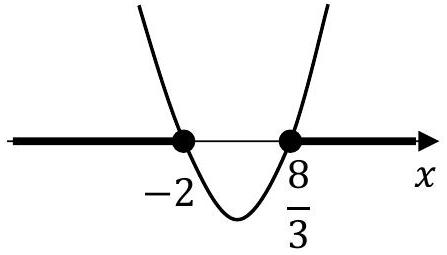
\includegraphics[max width=\textwidth, center]{2025_02_07_191ba7668814b12476d0g-13}
\end{itemize}

\section*{Uwagi:}
\begin{enumerate}
  \item Jeżeli zdający, realizując pierwszy etap rozwiązania zadania, popełni błędy (ale otrzyma dwa różne pierwiastki) i konsekwentnie do popełnionych błędów zapisze zbiór rozwiązań nierówności, to otrzymuje 1 punkt za całe rozwiązanie.
  \item Jeżeli zdający wyznacza pierwiastki trójmianu kwadratowego w przypadku, gdy błędnie obliczony przez zdającego wyróżnik $\Delta$ jest ujemny, to otrzymuje $\mathbf{0}$ punktów za całe rozwiązanie.
  \item Jeżeli zdający, rozpoczynając realizację pierwszego etapu rozwiązania, rozpatruje inny niż podany w zadaniu trójmian kwadratowy, który nie wynika z błędu przekształcenia (np. $3 x^{2}-2 x-9$ ) i w konsekwencji rozpatruje inną nierówność (np. $3 x^{2}-2 x-9 \geq 0$ ), to oznacza, że nie podjął realizacji 1. etapu rozwiązania i otrzymuje $\mathbf{0}$ punktów za całe rozwiązanie.
  \item Akceptowane jest zapisanie pierwiastków trójmianu w postaci $a+b \sqrt{c}$, gdzie $a, b, c$ są liczbami wymiernymi.
  \item Jeżeli zdający poda zbiór rozwiązań w postaci graficznej z poprawnie zaznaczonymi końcami przedziałów oraz zapisze: $x \in(-\infty,-2) \cup\left(\frac{8}{3},+\infty\right)$, to otrzymuje 1 punkt za całe rozwiązanie.
\end{enumerate}

\section*{Kryteria uwzględniające specyficzne trudności w uczeniu się matematyki}
Jeśli zdający pomyli porządek liczb na osi liczbowej, np. zapisze zbiór rozwiązań nierówności w postaci $\left(-\infty, \frac{8}{3}\right\rangle \cup\langle-2,+\infty),\left(+\infty, \frac{8}{3}\right\rangle \cup\langle-2,-\infty)$, to otrzymuje 2 punkty.

\section*{Przykładowe pełne rozwiązanie}
\section*{Pierwszy etap rozwiązania}
Zapisujemy nierówność w postaci $3 x^{2}-2 x-16 \geq 0$ i obliczamy pierwiastki trójmianu $3 x^{2}-2 x-16$.\\
Obliczamy wyróżnik tego trójmianu: $\Delta=196$ i stąd $x_{1}=-2$ oraz $x_{2}=\frac{8}{3}$\\
ALBO\\
podajemy pierwiastki trójmianu bezpośrednio, zapisując je lub zaznaczając je na wykresie:\\
$x_{1}=-2$ oraz $x_{2}=\frac{8}{3}$.

\section*{Drugi etap rozwiązania}
Podajemy zbiór rozwiązań nierówności: $(-\infty,-2\rangle \cup\left\langle\frac{8}{3},+\infty\right)$ lub $x \in(-\infty,-2\rangle \cup\left\langle\frac{8}{3},+\infty\right)$ lub zaznaczamy zbiór rozwiązań na osi liczbowej\\
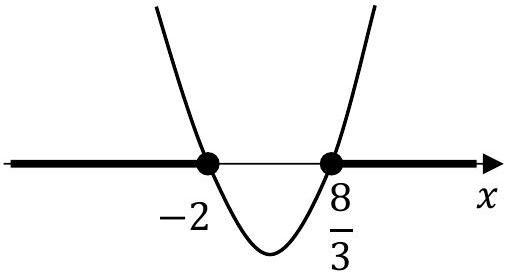
\includegraphics[max width=\textwidth, center]{2025_02_07_191ba7668814b12476d0g-14}

Zadanie 30. (0-2)

\begin{center}
\begin{tabular}{|l|l|}
\hline
\multicolumn{2}{|c|}{Wymagania egzaminacyjne 2022} \\
\hline
\multicolumn{1}{|c|}{Wymaganie ogólne} & \multicolumn{1}{c|}{Wymaganie szczegółowe} \\
\hline
III. Modelowanie matematyczne. & Zdający: \\
 & \begin{tabular}{l}
5.3) stosuje wzór na $n$-ty wyraz i na sumę \\
 \\
 \\
 \\
 \\
 \\
 \\
arytmetycznego. \\
\hline
\end{tabular} \\
\hline
\end{tabular}
\end{center}

\section*{Zasady oceniania}
\section*{Zdający otrzymuje 1 pkt gdy:}
\begin{itemize}
  \item zapisze równania wynikające z zastosowania poprawnych wzorów na $n$-ty wyraz ciągu arytmetycznego i sumę $n$ początkowych wyrazów ciągu arytmetycznego, np.
\end{itemize}

$$
a_{4}=a_{1}+3 r \text { i } S_{100}=\frac{2 a_{1}+(100-1) \cdot r}{2} \cdot 100
$$

lub

$$
a_{4}=a_{1}+3 r \text { i } a_{100}=a_{1}+99 r \text { i } S_{100}=\frac{a_{1}+a_{100}}{2} \cdot 100
$$

ALBO

\begin{itemize}
  \item poda/obliczy różnicę $r$ ciągu arytmetycznego $\left(a_{n}\right): r=3$ lub przyjmuje wrozwiązaniu, że $r=3$.
\end{itemize}

\section*{Zdający otrzymuje}
gdy obliczy sumę stu początkowych kolejnych wyrazów ciągu $\left(a_{n}\right): S_{100}=14750$.

\section*{Uwagi:}
\begin{enumerate}
  \item Jeśli zdający błędnie obliczy $r$ i konsekwentnie do otrzymanej wartości $r$ obliczy sumę stu początkowych wyrazów ciągu $\left(a_{n}\right)$, to otrzymuje 1 punkt za całe rozwiązanie.
  \item Jeśli zdający myli ciąg arytmetyczny z geometrycznym, to otrzymuje $\mathbf{0}$ punktów za całe rozwiązanie.
\end{enumerate}

\section*{Przykładowe pełne rozwiązania}
\section*{Sposób 1.}
Korzystamy ze wzoru na $n$-ty wyraz ciągu arytmetycznego i zapisujemy wzór na $a_{4}$ :

$$
a_{4}=a_{1}+3 \cdot r
$$

Zatem $8=-1+3 r$, więc $r=3$.\\
Korzystamy ze wzoru na sumę $n$ początkowych wyrazów ciągu arytmetycznego i obliczamy $S_{100}$ :

$$
S_{100}=\frac{2 a_{1}+(100-1) \cdot r}{2} \cdot 100=\frac{-2+297}{2} \cdot 100=14750
$$

\section*{Sposób 2.}
Korzystamy ze wzoru na $n$-ty wyraz ciągu arytmetycznego i zapisujemy wzór na czwarty wyraz tego ciągu:

$$
a_{4}=a_{1}+3 \cdot r
$$

gdzie $r$ oznacza różnicę ciągu.\\
Podstawiamy $a_{1}=-1$ oraz $a_{4}=8$ i otrzymujemy równanie $8=-1+3 r$, skąd $r=3$.\\
Sumę $n$ początkowych wyrazów ciągu arytmetycznego obliczymy ze wzoru

$$
S_{n}=\frac{a_{1}+a_{n}}{2} \cdot n
$$

Obliczamy setny wyraz ciągu $\left(a_{n}\right)$ :

$$
a_{100}=a_{1}+99 \cdot r=-1+99 \cdot 3=296
$$

Zatem suma stu początkowych wyrazów tego ciągu jest równa

$$
S_{100}=\frac{-1+296}{2} \cdot 100=295 \cdot 50=14750
$$

\section*{Zadanie 31. (0-2)}
\begin{center}
\begin{tabular}{|l|l|}
\hline
\multicolumn{2}{|c|}{Wymagania egzaminacyjne 2022} \\
\hline
\multicolumn{1}{|c|}{Wymaganie ogólne} & \multicolumn{1}{|c|}{Wymaganie szczegółowe} \\
\hline
V. Rozumowanie i argumentacja. & \begin{tabular}{l}
Zdający: \\
 \\
 \\
 \\
 \\
 \\
 \\
 \\
\hline
\end{tabular} 2.1) używa wzorów skróconego mnożenia $(a \pm b)^{2}[\ldots]$. \\
\hline
\end{tabular}
\end{center}

\section*{Zasady oceniania}
\section*{Zdający otrzymuje \\
 1 pkt}
gdy:

\begin{itemize}
  \item przekształci nierówność $\frac{a^{2}+b^{2}}{2}>\left(\frac{a+b}{2}\right)^{2}$ do postaci równoważnej $(a-b)^{2}>0$ lub $a^{2}+b^{2}>2 a b$ (dla sposobu 1.), o ile na tym zakończy lub $z$ tej postaci wyciągnie wniosek\\
ALBO
  \item wykorzysta założenie $a \neq b$ (lub równoważnie $(a-b)^{2}>0$ ) i zapisze $a^{2}+b^{2}>2 a b$ (dla sposobu 2.),\\
ALBO
  \item wykorzysta założenie $a \neq b$ oraz zapisze nierówność pomiędzy średnimi: kwadratową i arytmetyczną, dla liczb nieujemnych (dla sposobu 3.).
\end{itemize}

Zdający otrzymuje\\
gdy przeprowadzi pełne rozumowanie, tzn.

\begin{itemize}
  \item spełni kryterium określone w zasadach oceniania w pierwszej kropce za 1 pkt oraz sformułuje poprawny wniosek z powołaniem się na założenie
\end{itemize}

ALBO

\begin{itemize}
  \item spełni kryterium określone w zasadach oceniania w drugiej kropce za 1 pkt oraz doprowadzi nierówność do postaci tezy,
\end{itemize}

\section*{ALBO}
\begin{itemize}
  \item w sposobie 3., opierając się na nierówności pomiędzy średnią kwadratową i średnią arytmetyczną, wykaże prawdziwość nierówności $\frac{a^{2}+b^{2}}{2}>\left(\frac{a+b}{2}\right)^{2}$ dla każdych liczb rzeczywistych $a$ i $b$ takich, że $a \neq b$.
\end{itemize}

\section*{Uwaga:}
Jeśli zdający sprawdza prawdziwość nierówności tylko dla wybranych wartości $a$ i $b$, to otrzymuje 0 punktów za całe rozwiązanie.

\section*{Przykładowe pełne rozwiązania}
\section*{Sposób 1.}
Przekształcamy równoważnie nierówność $\frac{a^{2}+b^{2}}{2}>\left(\frac{a+b}{2}\right)^{2}$ :

$$
\begin{gathered}
\frac{a^{2}+b^{2}}{2}>\left(\frac{a+b}{2}\right)^{2} \\
\frac{a^{2}+b^{2}}{2}>\frac{a^{2}+2 a b+b^{2}}{4} \\
2 a^{2}+2 b^{2}>a^{2}+2 a b+b^{2} \\
a^{2}-2 a b+b^{2}>0 \\
(a-b)^{2}>0
\end{gathered}
$$

Z założenia wiadomo, że $b \neq a$, więc $(a-b)^{2}$ jest liczbą dodatnią jako kwadrat liczby rzeczywistej $a-b$ różnej od zera. Ponieważ nierówność $(a-b)^{2}>0$ jest prawdziwa, więc nierówność $\frac{a^{2}+b^{2}}{2}>\left(\frac{a+b}{2}\right)^{2}$ również jest prawdziwa. To należało pokazać.

Sposób 2. (od założenia do tezy)\\
Z założenia wiadomo, że $a \neq b$, zatem różnica $a-b \neq 0$. Stąd wynika, że ( $a-b)^{2}$ jest liczbą dodatnią. Nierówność $(a-b)^{2}>0$ jest równoważna nierówności

$$
a^{2}+b^{2}>2 a b
$$

Zauważmy teraz, że tożsamość $(a+b)^{2}=a^{2}+2 a b+b^{2}$ można zapisać w równoważnej postaci

$$
(a+b)^{2}-\left(a^{2}+b^{2}\right)=2 a b
$$

Nierówność $a^{2}+b^{2}>2 a b$ zapisujemy więc w postaci

$$
a^{2}+b^{2}>(a+b)^{2}-\left(a^{2}+b^{2}\right)
$$

Zatem

$$
2\left(a^{2}+b^{2}\right)>(a+b)^{2}
$$

Dzielimy obie strony tej nierówności przez 4 i otrzymujemy nierówność

$$
\frac{a^{2}+b^{2}}{2}>\frac{(a+b)^{2}}{4}
$$

Ta nierówność jest równoważna nierówności

$$
\frac{a^{2}+b^{2}}{2}>\left(\frac{a+b}{2}\right)^{2}
$$

zapisanej w tezie twierdzenia. To należało pokazać.\\
Sposób 3. (nierówność między średnimi)\\
Obie strony nierówności $\frac{a^{2}+b^{2}}{2}>\left(\frac{a+b}{2}\right)^{2}$ są nieujemne, więc pierwiastkując je, otrzymujemy nierówność równoważną

$$
\sqrt{\frac{a^{2}+b^{2}}{2}}>\left|\frac{a+b}{2}\right|
$$

czyli

$$
\sqrt{\frac{a^{2}+b^{2}}{2}}>\frac{|a+b|}{2}
$$

Wykażemy, że jest ona prawdziwa dla każdych liczb rzeczywistych $a$ i $b$ takich, że $a \neq b$. Dla liczb rzeczywistych $a$ i $b$ liczby $|a|$ i $|b|$ są nieujemne, więc prawdziwa jest nierówność między średnią kwadratową i średnią arytmetyczną

$$
\sqrt{\frac{|a|^{2}+|b|^{2}}{2}} \geq \frac{|a|+|b|}{2}
$$

przy czym równość zachodzi tylko wtedy, gdy $|a|=|b|$.\\
Ponieważ $x^{2}=|x|^{2},|x|+|y| \geq|x+y|,|x| \geq x$ dla każdych liczb rzeczywistych $x$ oraz $y$, więc otrzymujemy

$$
\sqrt{\frac{a^{2}+b^{2}}{2}}=\sqrt{\frac{|a|^{2}+|b|^{2}}{2}} \geq \frac{|a|+|b|}{2} \geq \frac{|a+b|}{2} \geq \frac{a+b}{2}
$$

Pozostaje wykazać, że jeżeli $a \neq b$, to prawdziwa jest nierówność ostra

$$
\sqrt{\frac{a^{2}+b^{2}}{2}}>\frac{|a+b|}{2}
$$

Gdy $|a| \neq|b|$, to prawdziwość nierówności ostrej wynika z nierówności między średnią kwadratową i średnią arytmetyczną. Równość $|a|=|b|$ oznacza, że liczby $a$ i $b$ są równe lub przeciwne. Jednak z założenia liczby $a$ i $b$ są różne. Jeśli są przeciwne, czyli\\
$a+b=0$, to wtedy prawa strona tej nierówności jest równa zero, natomiast lewa strona jest dodatnia - zerem byłaby tylko wtedy, gdyby $a=b=0$, co jest sprzeczne z założeniem $a \neq b$.

Zadanie 32. (0-2)

\begin{center}
\begin{tabular}{|l|l|}
\hline
\multicolumn{2}{|c|}{Wymagania egzaminacyjne 2022} \\
\hline
\multicolumn{1}{|c|}{Wymaganie ogólne} & \multicolumn{1}{c|}{Wymagania szczegółowe} \\
\hline
IV. Użycie i tworzenie strategii. & Zdający: \\
 & 6.3) stosuje proste zależności między \\
 & funkcjami trygonometrycznymi $[. .] ;$. \\
 & 6.4) znając wartość jednej z funkcji: sinus \\
 & lub cosinus, wyznacza wartości \\
 & pozostałych funkcji tego samego kąta. \\
\hline
\end{tabular}
\end{center}

\section*{Zasady oceniania}
\section*{Zdający otrzymuje}
gdy:

\begin{itemize}
  \item zapisze układ równań $\frac{\sin \alpha}{\cos \alpha}=2$ i $\sin ^{2} \alpha+\cos ^{2} \alpha=1$ (lub jedno równanie równoważne temu układowi, np. $(2 \cos \alpha)^{2}+\cos ^{2} \alpha=1, \sin ^{2} \alpha+\left(\frac{1}{2} \sin \alpha\right)^{2}=1$, $\left.\sin ^{2} \alpha=4\left(1-\sin ^{2} \alpha\right)\right)$\\
ALBO
  \item narysuje trójkąt prostokątny, zaznaczy na rysunku kąt $\alpha$ (lub z rozwiązania wynika, że poprawnie go interpretuje) i zapisze relację między przyprostokątnymi tego trójkąta wynikającą z warunku zadania oraz relację między długościami boków trójkąta wynikającą z twierdzenia Pitagorasa.
\end{itemize}

\section*{Zdający otrzymuje}
gdy spełni kryterium za 1 punkt z zasad oceniania i obliczy wartość wyrażenia $\sin ^{2} \alpha$ : $\sin ^{2} \alpha=\frac{4}{5}$.

\section*{Uwaga:}
Jeśli zdający odczyta przybliżoną wartość kąta, dla którego $\operatorname{tg} \alpha=2$ ( $\alpha=63^{\circ}$ lub $\alpha=64^{\circ}$ ) i na tej podstawie oblicza $\sin ^{2} \alpha$, stosując poprawnie regułę zaokrąglania, to otrzymuje 1 punkt za całe rozwiązanie.

\section*{Przykładowe pełne rozwiązania}
\section*{Sposób 1.}
Ponieważ $\operatorname{tg} \alpha=2$, więc $\frac{\sin \alpha}{\cos \alpha}=2$ i stąd $\sin \alpha=2 \cos \alpha$. Korzystając z tego związku i tożsamości $\sin ^{2} \alpha+\cos ^{2} \alpha=1$, otrzymujemy

$$
\begin{gathered}
(2 \cos \alpha)^{2}+\cos ^{2} \alpha=1 \\
5 \cos ^{2} \alpha=1 \\
\cos ^{2} \alpha=\frac{1}{5}
\end{gathered}
$$

Ponownie korzystamy z tożsamości $\sin ^{2} \alpha+\cos ^{2} \alpha=1$ i obliczamy $\sin ^{2} \alpha$ :

$$
\begin{gathered}
\sin ^{2} \alpha+\cos ^{2} \alpha=1 \\
\sin ^{2} \alpha+\frac{1}{5}=1 \\
\sin ^{2} \alpha=\frac{4}{5}
\end{gathered}
$$

Sposób 2.\\
Niech $A B C$ będzie trójkątem prostokątnym, w którym $|\Varangle C A B|=90^{\circ}$ oraz $|\Varangle A B C|=\alpha$.\\
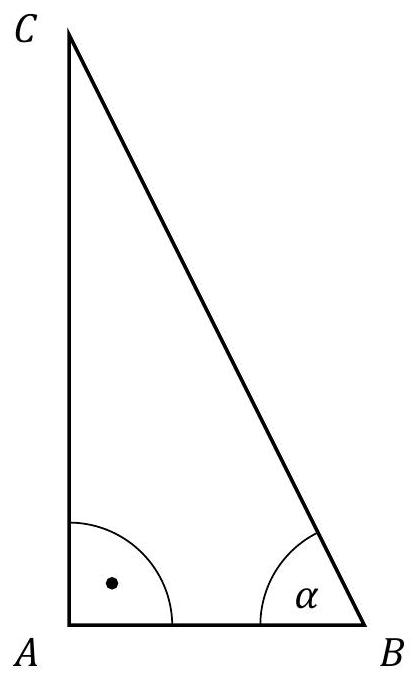
\includegraphics[max width=\textwidth, center]{2025_02_07_191ba7668814b12476d0g-20}

Ponieważ $\operatorname{tg} \alpha=2$, więc $\frac{|A C|}{|A B|}=2$, czyli $|A C|=2 \cdot|A B|$. Wyznaczamy długość odcinka $B C$ w zależności od długości odcinka $A B$. Korzystamy z twierdzenia Pitagorasa i otrzymujemy

$$
\begin{gathered}
|B C|^{2}=|A C|^{2}+|A B|^{2} \\
|B C|^{2}=(2 \cdot|A B|)^{2}+|A B|^{2} \\
|B C|^{2}=5 \cdot|A B|^{2} \\
|B C|=\sqrt{5} \cdot|A B|
\end{gathered}
$$

Zatem $\sin ^{2} \alpha=\left(\frac{|A C|}{|B C|}\right)^{2}=\left(\frac{2 \cdot|A B|}{\sqrt{5} \cdot|A B|}\right)^{2}=\frac{4}{5}$.

Zadanie 33. (0-2)

\begin{center}
\begin{tabular}{|c|c|}
\hline
\multicolumn{2}{|c|}{Wymagania egzaminacyjne 2022} \\
\hline
Wymaganie ogólne & Wymaganie szczegółowe \\
\hline
IV. Użycie i tworzenie strategii. & \begin{tabular}{l}
Zdający: \\
7.3) rozpoznaje trójkąty podobne i wykorzystuje cechy podobieństwa trójkątów. \\
\end{tabular} \\
\hline
\end{tabular}
\end{center}

\section*{Zasady oceniania}
Zdający otrzymuje

\begin{itemize}
  \item zauważy, że trójkąt $A B D$ jest równoramienny i zapisze $|A B|=|A D|$ lub $|\Varangle A B D|=|\Varangle A D B|$\\
ALBO
  \item zapisze, że $|\Varangle A D B|=|\Varangle B A C|$,
\end{itemize}

ALBO

\begin{itemize}
  \item zapisze, że $|\Varangle B A D|=|\Varangle A C B|$.
\end{itemize}

\section*{Zdający otrzymuje}
gdy zastosuje poprawną metodę i otrzyma poprawny wynik: $|\Varangle B A C|=72^{\circ}$.

\section*{Uwagi:}
\begin{enumerate}
  \item Jeżeli zdający przyjmuje, że odcinek $A D$ jest prostopadły do boku $B C$ i korzysta z tego w rozwiązaniu, to otrzymuje 0 punktów za całe rozwiązanie.
  \item Jeśli zdający zapisze tylko $|\Varangle B A C|=72^{\circ}$, to otrzymuje 1 punkt za całe rozwiązanie.
\end{enumerate}

\section*{Przykładowe pełne rozwiązania}
\section*{Sposób 1.}
Oznaczmy przez $2 \alpha$ miarę kąta $B A C$. Odcinek $A D$ jest zawarty w dwusiecznej kąta $B A C$, więc $|\Varangle B A D|=|\Varangle C A D|=\alpha$.\\
Ponieważ $|A C|=|B C|$, więc $|\Varangle A B C|=2 \alpha$ (zobacz rysunek obok).\\
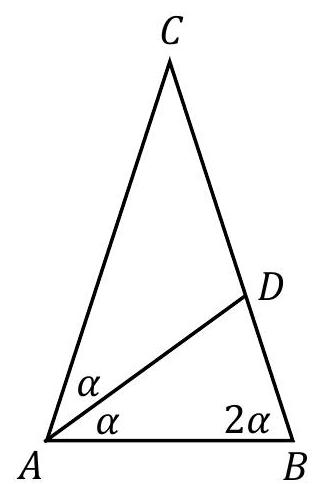
\includegraphics[max width=\textwidth, center]{2025_02_07_191ba7668814b12476d0g-21}

Trójkąty $A B C$ i $B D A$ są podobne, miary kątów przy podstawie $A B$ trójkąta $A B C$ są równe $2 \alpha$ i ponadto $|\Varangle A B D|=2 \alpha$, więc trójkąt $A B D$ jest równoramienny oraz $|\Varangle A D B|=|\Varangle A B D|=2 \alpha$.\\
Stosujemy do trójkąta $A B D$ twierdzenie o sumie miar kątów wewnętrznych trójkąta i otrzymujemy

$$
|\Varangle B A D|+|\Varangle A B D|+|\Varangle A D B|=180^{\circ}
$$

$$
\begin{gathered}
\alpha+2 \alpha+2 \alpha=180^{\circ} \\
5 \alpha=180^{\circ} \\
\alpha=36^{\circ}
\end{gathered}
$$

Zatem $|\Varangle B A C|=2 \alpha=2 \cdot 36^{\circ}=72^{\circ}$.\\
Sposób 2.\\
Oznaczmy przez $2 \alpha$ miarę kąta $B A C$. Odcinek $A D$ jest zawarty w dwusiecznej kąta $B A C$, więc $|\Varangle B A D|=|\Varangle C A D|=\alpha$. Ponieważ $|A C|=|B C|$, więc $|\Varangle A B C|=2 \alpha$ (zobacz rysunek).\\
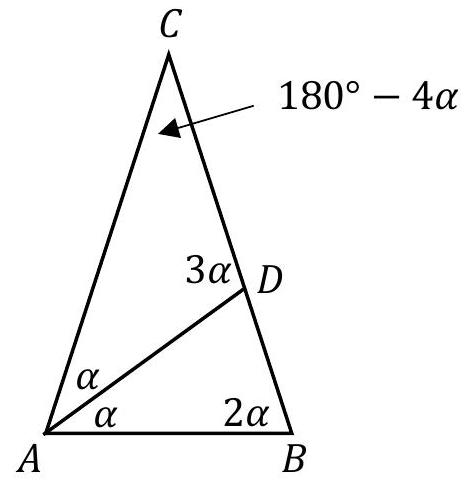
\includegraphics[max width=\textwidth, center]{2025_02_07_191ba7668814b12476d0g-22}

Stosujemy do trójkąta $A B D$ twierdzenie o sumie miar kątów wewnętrznych trójkąta i otrzymujemy

$$
|\Varangle A D B|=180^{\circ}-(\alpha+2 \alpha)=180^{\circ}-3 \alpha
$$

Kąty $A D C$ i $A D B$ są przyległe, zatem $|\Varangle A D C|=3 \alpha$.\\
Stosujemy do trójkąta $A D C$ twierdzenie o sumie miar kątów wewnętrznych trójkąta i otrzymujemy

$$
|\Varangle A C D|=180^{\circ}-4 \alpha
$$

Trójkąty $A B C$ i $B D A$ są podobne, miary kątów między ramionami są równe, więc

$$
\begin{gathered}
180^{\circ}-4 \alpha=\alpha \\
5 \alpha=180^{\circ} \\
\alpha=36^{\circ}
\end{gathered}
$$

Zatem $|\Varangle B A C|=2 \alpha=2 \cdot 36^{\circ}=72^{\circ}$.

Zadanie 34. (0-2)

\begin{center}
\begin{tabular}{|l|l|}
\hline
\multicolumn{2}{|c|}{Wymagania egzaminacyjne 2022} \\
\hline
\multicolumn{1}{|c|}{Wymaganie ogólne} & \multicolumn{1}{c|}{Wymaganie szczegółowe} \\
\hline
III. Modelowanie matematyczne. & Zdający: \\
 & 10.2) oblicza prawdopodobieństwa \\
 & w prostych sytuacjach, stosując klasyczną \\
 & definicję prawdopodobieństwa. \\
\hline
\end{tabular}
\end{center}

\section*{Zasady oceniania}
\section*{Zdający otrzymuje}
\begin{itemize}
  \item wypisze wszystkie zdarzenia elementarne lub obliczy/poda ich liczbę: $|\Omega|=9.9$
\end{itemize}

ALBO

\begin{itemize}
  \item wypisze (zaznaczy w tabeli) wszystkie zdarzenia elementarne sprzyjające zdarzeniu $A$ i nie wypisze żadnego niewłaściwego:
\end{itemize}

$$
(3,8),(4,6),(6,4),(8,3),
$$

ALBO

\begin{itemize}
  \item poda liczbę wszystkich zdarzeń elementarnych sprzyjających zdarzeniu $A:|A|=4$, ALBO
  \item sporządzi fragment drzewa stochastycznego, które zawiera wszystkie gałęzie sprzyjające zdarzeniu $A$ oraz zapisze prawdopodobieństwo $\frac{1}{9}$ na co najmniej jednym odcinku każdego z etapów doświadczenia,\\
ALBO
  \item zapisze tylko $P(A)=\frac{4}{81}$.
\end{itemize}

\section*{Zdający otrzymuje}
gdy spełni warunki określone w zasadach oceniania za 1 pkt oraz zastosuje poprawną metodę obliczenia prawdopodobieństwa zdarzenia $A$ i uzyska poprawny wynik:\\
$P(A)=\frac{|A|}{|\Omega|}=\frac{4}{81}$.

\section*{Uwagi:}
\begin{enumerate}
  \item Jeżeli zdający zapisuje tylko liczby 4 lub 81 i $z$ rozwiązania nie wynika znaczenie tych liczb, to otrzymuje $\mathbf{0}$ punktów za całe rozwiązanie.
  \item Jeżeli zdający sporządzi jedynie tabelę o 81 pustych polach, to otrzymuje $\mathbf{0}$ punktów za całe rozwiązanie.
\end{enumerate}

\section*{Przykładowe pełne rozwiązania}
Sposób 1. (klasyczna definicja prawdopodobieństwa)\\
Zdarzeniami elementarnymi są wszystkie uporządkowane pary liczb ( $a, b$ ), gdzie $a, b \in M$.

Liczba wszystkich zdarzeń elementarnych jest równa $|\Omega|=9 \cdot 9=81$.\\
Zdarzeniu $A$ sprzyjają następujące zdarzenia elementarne:\\
$(3,8),(4,6),(6,4),(8,3)$,\\
więc $|A|=4$.\\
Prawdopodobieństwo zdarzenia $A$ jest równe: $P(A)=\frac{|A|}{|\Omega|}=\frac{4}{81}$.

\section*{Sposób 2.}
Zdarzeniami elementarnymi są wszystkie uporządkowane pary liczb $(a, b)$, gdzie $a, b \in M$. Jest to model klasyczny. Budujemy tabelę ilustrującą sytuację opisaną w zadaniu.

I losowanie\\
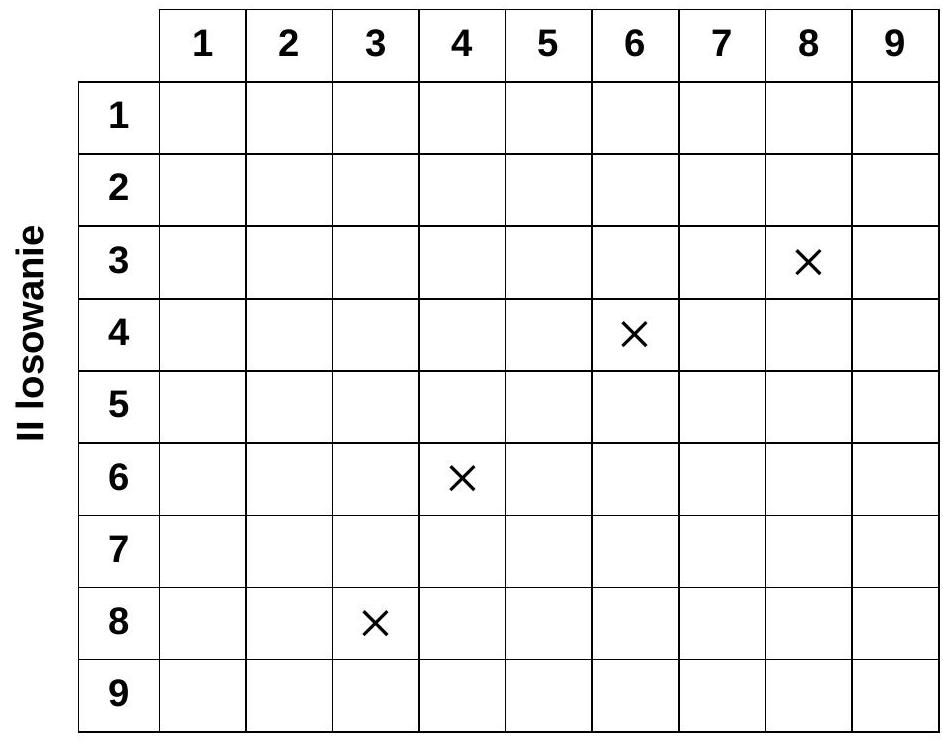
\includegraphics[max width=\textwidth, center]{2025_02_07_191ba7668814b12476d0g-24}

Symbolem $\times$ oznaczono pola odpowiadające zdarzeniom elementarnym sprzyjającym zdarzeniu $A$.\\
Wszystkich zdarzeń elementarnych w tym doświadczeniu jest 81.\\
Liczba wszystkich zdarzeń elementarnych sprzyjających zdarzeniu $A$ jest równa 4.\\
Stąd $P(A)=\frac{|A|}{|\Omega|}=\frac{4}{81}$.

Sposób 3. (drzewo stochastyczne)\\
Rysujemy fragment drzewa stochastycznego rozważanego doświadczenia z uwzględnieniem wszystkich istotnych gałęzi.\\
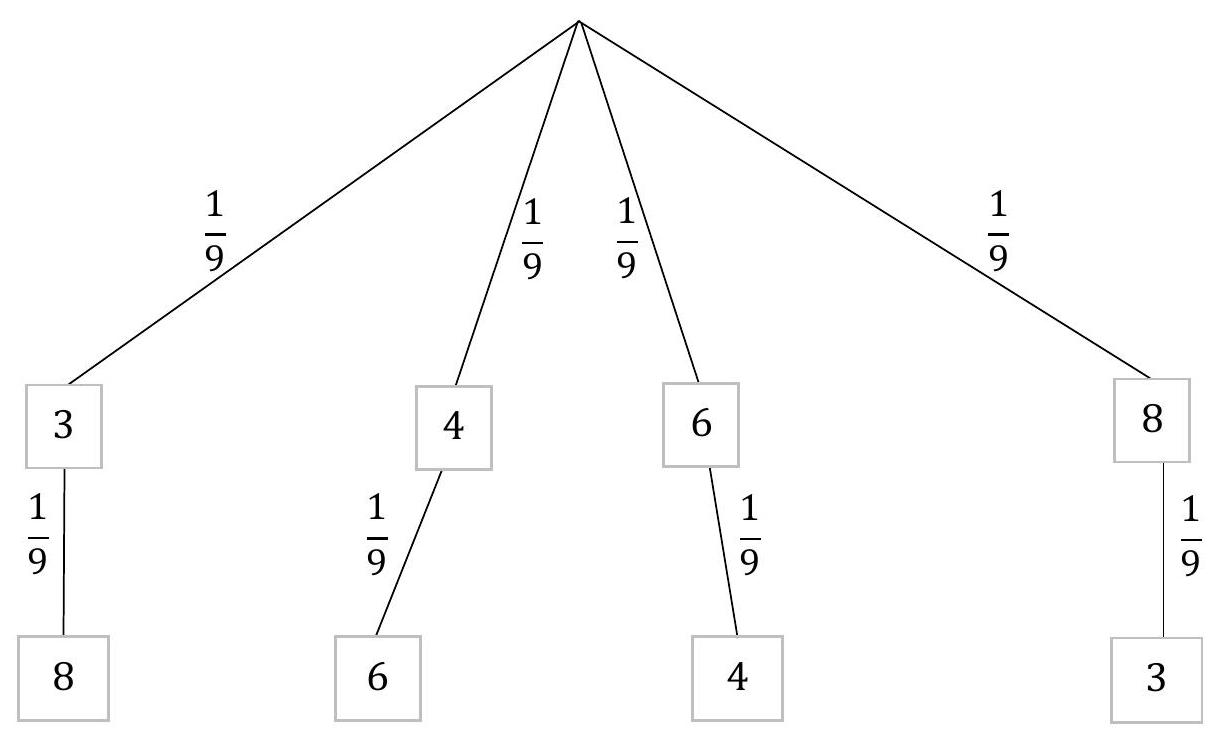
\includegraphics[max width=\textwidth, center]{2025_02_07_191ba7668814b12476d0g-25}

Prawdopodobieństwo zdarzenia $A$ jest równe

$$
P(A)=\frac{1}{9} \cdot \frac{1}{9}+\frac{1}{9} \cdot \frac{1}{9}+\frac{1}{9} \cdot \frac{1}{9}+\frac{1}{9} \cdot \frac{1}{9}=\frac{4}{81}
$$

Zadanie 35. (0-5)

\begin{center}
\begin{tabular}{|l|l|}
\hline
\multicolumn{2}{|c|}{Wymagania egzaminacyjne 2022} \\
\hline
\multicolumn{1}{|c|}{Wymaganie ogólne} & \multicolumn{1}{c|}{Wymaganie szczegółowe} \\
\hline
III. Modelowanie matematyczne. & \begin{tabular}{l}
Zdajacy: \\
 \\
 \\
 \\
 \\
 \\
 \\
\hline
\end{tabular}\begin{tabular}{l}
4.9) wyznacza wzór funkcji kwadratowej na \\
podstawie pewnych informacji o funkcji lub \\
o jej wykresie. \\
\end{tabular} \\
\hline
\end{tabular}
\end{center}

Zasady oceniania dla sposobów 1.-5.\\
Zdający otrzymuje\\
gdy:

\begin{itemize}
  \item zapisze wzór funkcji $f$ w postaci $f(x)=a(x+5)(x-3)$
\end{itemize}

ALBO

\begin{itemize}
  \item poda/obliczy odciętą $p$ wierzchołka paraboli: $p=-1$,
\end{itemize}

ALBO

\begin{itemize}
  \item zapisze jedno równanie z niewiadomymi $a, b$ oraz $c$ wynikające z treści zadania, np.
\end{itemize}

$$
\begin{aligned}
& a \cdot(-5)^{2}+b \cdot(-5)+c=0 \text { lub } a \cdot 3^{2}+b \cdot 3+c=0, \text { lub } 6=\frac{-\left(b^{2}-4 a c\right)}{4 a}, \\
& \text { lub }-\frac{b}{a}=-2, \text { lub } \frac{c}{a}=-15,
\end{aligned}
$$

ALBO

\begin{itemize}
  \item zapisze, że rzędna $q$ wierzchołka paraboli jest równa 6: $q=6$.
\end{itemize}

\section*{Zdający otrzymuje}
gdy:

\begin{itemize}
  \item zapisze wzór funkcji $f$ w postaci $f(x)=a(x+5)(x-3)$ lub w postaci $f(x)=a x^{2}+2 a x-15 a$ oraz zapisze, że rzędna wierzchołka paraboli jest równa 6 ALBO
  \item zapisze wzór funkcji $f$ w postaci $f(x)=a(x+1)^{2}+6$,
\end{itemize}

\section*{ALBO}
\begin{itemize}
  \item poda/obliczy odciętą wierzchołka paraboli i poda rzędną wierzchołka paraboli: $p=-1, q=6$,
\end{itemize}

ALBO

\begin{itemize}
  \item zapisze układ dwóch równań z trzema niewiadomymi $a, b, c, z$ których jedno jest jednym z równań\\
$6=\frac{-\left(b^{2}-4 a c\right)}{4 a}$ lub $6=a \cdot(-1)^{2}+b \cdot(-1)+c$,\\
natomiast drugie jest jednym $z$ równań\\
$a \cdot(-5)^{2}+b \cdot(-5)+c=0$ lub $a \cdot 3^{2}+b \cdot 3+c=0$, lub $-\frac{b}{2 a}=-1$, lub $-\frac{b}{a}=-2$, lub $\frac{c}{a}=-15$,\\
ALBO
  \item zapisze równanie $a(x+5)(x-3)-6=0$ (dla sposobu 5.).
\end{itemize}

Zdający otrzymuje gdy:

\begin{itemize}
  \item zapisze równanie z jedną niewiadomą $a, \mathrm{np}$.\\
$6=a(-1+5)(-1-3)$ lub $0=a(3+1)^{2}+6$, lub $0=a(-5+1)^{2}+6$\\
ALBO
  \item zapisze układ trzech niezależnych równań z trzema niewiadomymi $a, b, c$ prowadzący do obliczenia wartości współczynników $a, b$ oraz $c, \mathrm{np}$.\\
$a \cdot(-5)^{2}+b \cdot(-5)+c=0$ i $a \cdot 3^{2}+b \cdot 3+c=0$ i $6=\frac{-\left(b^{2}-4 a c\right)}{4 a}$ LUB\\
$-\frac{b}{a}=-2 \quad$ i $\frac{c}{a}=-15 \quad$ i $6=\frac{-\left(b^{2}-4 a c\right)}{4 a}$,\\
LUB\\
$a \cdot(-5)^{2}+b \cdot(-5)+c=0$ i $a \cdot 3^{2}+b \cdot 3+c=0$ i $6=a \cdot(-1)^{2}+b \cdot(-1)+c$, LUB
\end{itemize}

$$
-\frac{b}{2 a}=-1 \text { i } a \cdot 3^{2}+b \cdot 3+c=0 \text { i } 6=a \cdot(-1)^{2}+b \cdot(-1)+c,
$$

LUB\\
$a \cdot(-5)^{2}+b \cdot(-5)+c=0$ i $-\frac{b}{2 a}=-1$ i $6=a \cdot(-1)^{2}+b \cdot(-1)+c$,\\
ALBO

\begin{itemize}
  \item uzależni współczynniki $b$ oraz $c$ od $a$ i zapisze współrzędne wierzchołka paraboli, np. $b=2 a$ oraz $c=-15 a$ oraz $W=(-1,6)$,\\
ALBO
  \item zapisze wzór funkcji w postaci $f(x)=a x^{2}+2 a x-15 a$ oraz zapisze współrzędne wierzchołka paraboli: $W=(-1,6)$\\
(lub zapisze wzór funkcji w postaci $f(x)=a x^{2}+2 a x+a+6$ oraz zapisze równość $f(-5)=0$ lub $f(3)=0)$,\\
ALBO
  \item zapisze wzór funkcji w postaciach\\
$f(x)=a x^{2}-2 a p x+a p^{2}+6$ i $f(x)=a x^{2}+2 a x-15 a$\\
oraz zapisze układ równań $-2 a p=2 a$ i $a p^{2}+6=-15 a$,\\
ALBO
  \item uzależni współczynniki $b$ oraz $c$ od $a$ (np. $b=2 a$ oraz $c=-15 a$ ) oraz zapisze związki $\Delta=64 a^{2}$ i $q=6$,\\
ALBO
  \item zapisze, że wyróżnik trójmianu $a x^{2}+2 a x-15 a-6$ musi być równy 0 (dla sposobu 5.).
\end{itemize}

\section*{Zdający otrzymuje}
gdy:

\begin{itemize}
  \item zapisze wzór funkcji $f$ w postaci $f(x)=a(x+5)(x-3)$ i obliczy\\
współczynnik $a$ : $a=-\frac{3}{8}$\\
ALBO
  \item zapisze wzór funkcji $f$ w postaci $f(x)=a(x+1)^{2}+6$ i obliczy współczynnik $a$ : $a=-\frac{3}{8}$,\\
ALBO
  \item obliczy poprawnie tylko dwa współczynniki spośród $a, b$ oraz $c$, pomijając w obliczeniach trzeci współczynnik,\\
ALBO
  \item obliczy współczynniki $a, b$ oraz $c$, popełniając w trakcie rozwiązywania jedynie błędy rachunkowe.
\end{itemize}

\section*{Zdający otrzymuje}
gdy obliczy współczynniki $a, b$ oraz $c: a=-\frac{3}{8}, b=-\frac{3}{4}, c=\frac{45}{8}$.

\section*{Uwagi:}
\begin{enumerate}
  \item Jeśli zdający poprawnie obliczy/poda obie współrzędne wierzchołka paraboli, ale zapisze błędne równanie $0=a(3-1)^{2}+6$ lub $0=a(-5-1)^{2}+6$, a następnie konsekwentnie do popełnionego błędu rozwiąże zadanie do końca, to otrzymuje 3 punkty za całe rozwiązanie.
  \item Jeśli zdający poprawnie zidentyfikuje miejsca zerowe funkcji, ale zapisze błędne równanie $6=a(-1-5)(-1-3)$ i konsekwentnie do popełnionego błędu rozwiąże zadanie do końca, to otrzymuje 3 punkty za całe rozwiązanie.
  \item Jeśli zdający ustali poprawną wartość współczynnika $a$ i konsekwentnie rozwiąże zadanie do końca, nie popełniając błędu, to może otrzymać 5 punktów za całe rozwiązanie.
  \item Jeśli zdający przyjmie wspórrzędne wierzchołka paraboli $(6,-1)$ i konsekwentnie rozwiąże zadanie do końca, to otrzymuje 3 punkty za całe rozwiązanie.
\end{enumerate}

\section*{Przykładowe pełne rozwiązania}
\section*{Sposób 1.}
Ponieważ parabola, która jest wykresem funkcji $f$, przecina oś $O x$ układu współrzędnych w punktach $A=(-5,0)$ i $B=(3,0)$, więc pierwiastkami trójmianu są liczby $x_{1}=-5$ oraz $x_{2}=3$. Zatem wzór funkcji $f$ możemy zapisać w postaci iloczynowej $f(x)=a(x+5)(x-3)$.\\
Znając pierwiastki trójmianu, obliczamy odciętą $p$ wierzchołka tej paraboli

$$
p=\frac{x_{1}+x_{2}}{2}=\frac{-5+3}{2}=-1
$$

Ponieważ parabola ma z prostą o równaniu $y=6$ dokładnie jeden punkt wspólny, więc rzędna $q$ wierzchołka tej paraboli jest równa 6 . Podstawiając współrzędne wierzchołka paraboli do wzoru funkcji $f$, otrzymujemy

$$
\begin{gathered}
6=a(-1+5)(-1-3) \\
6=-16 a \\
a=-\frac{6}{16}=-\frac{3}{8}
\end{gathered}
$$

Zapisujemy funkcję kwadratową w postaci ogólnej

$$
f(x)=-\frac{3}{8}(x+5)(x-3)=-\frac{3}{8} x^{2}-\frac{3}{4} x+\frac{45}{8}
$$

Stąd odczytujemy wartości współczynników trójmianu: $a=-\frac{3}{8}, b=-\frac{3}{4}, c=\frac{45}{8}$.

\section*{Sposób 2.}
Ponieważ parabola, która jest wykresem funkcji $f$, przecina oś $O x$ układu współrzędnych w punktach $A=(-5,0)$ i $B=(3,0)$, więc pierwiastkami trójmianu są liczby $x_{1}=-5$ oraz $x_{2}=3$. Znając pierwiastki trójmianu, obliczamy odciętą $p$ wierzchołka tej paraboli

$$
p=\frac{x_{1}+x_{2}}{2}=\frac{-5+3}{2}=-1
$$

Ponieważ parabola ma z prostą o równaniu $y=6$ dokładnie jeden punkt wspólny, więc rzędna $q$ wierzchołka tej paraboli jest równa 6.\\
Zapisujemy wzór funkcji $f$ w postaci kanonicznej $f(x)=a(x+1)^{2}+6$.\\
Ponieważ $f(3)=0$, więc

$$
\begin{gathered}
0=a(3+1)^{2}+6 \\
0=16 a+6 \\
a=-\frac{6}{16}=-\frac{3}{8}
\end{gathered}
$$

Zatem $f(x)=-\frac{3}{8}(x+1)^{2}+6=-\frac{3}{8}\left(x^{2}+2 x+1\right)+6=-\frac{3}{8} x^{2}-\frac{3}{4} x+\frac{45}{8}$.\\
Stąd odczytujemy wartości współczynników trójmianu: $a=-\frac{3}{8}, b=-\frac{3}{4}, c=\frac{45}{8}$.

\section*{Sposób 3.}
Punkty $A=(-5,0)$ i $B=(3,0)$ należą do wykresu funkcji $f$, więc

$$
a \cdot(-5)^{2}+b \cdot(-5)+c=0 \quad \text { i } \quad a \cdot 3^{2}+b \cdot 3+c=0
$$

Odejmując stronami te dwa równania otrzymujemy

$$
\begin{gathered}
(25 a-5 b+c)-(9 a+3 b+c)=0 \\
16 a-8 b=0 \\
b=2 a
\end{gathered}
$$

Ponieważ parabola ma z prostą o równaniu $y=6$ dokładnie jeden punkt wspólny, więc rzędna $q$ wierzchołka paraboli jest równa 6. Zatem

$$
\begin{gathered}
q=\frac{-\Delta}{4 a} \\
6=\frac{-\left(b^{2}-4 a c\right)}{4 a}
\end{gathered}
$$

Podstawiamy do ostatniego równania w miejsce $b$ wyrażenie $2 a$ i otrzymujemy

$$
\begin{gathered}
6=\frac{-\left((2 a)^{2}-4 a c\right)}{4 a} \\
6=\frac{-4 a^{2}+4 a c}{4 a} \\
6=\frac{4 a(-a+c)}{4 a} \\
6=-a+c
\end{gathered}
$$

$$
c=6+a
$$

Z uzyskanych wcześniej równań $a \cdot 3^{2}+b \cdot 3+c=0, b=2 a$ i $c=6+a$ obliczamy $a$ :

$$
\begin{gathered}
a \cdot 3^{2}+2 a \cdot 3+6+a=0 \\
16 a=-6 \\
a=-\frac{6}{16}=-\frac{3}{8}
\end{gathered}
$$

Stąd $b=2 a=2 \cdot\left(-\frac{3}{8}\right)=-\frac{3}{4}$ oraz $c=6+a=6-\frac{3}{8}=\frac{45}{8}$.

\section*{Sposób 4.}
Ponieważ parabola, która jest wykresem funkcji $f$, przecina oś $O x$ układu współrzędnych w punktach $A=(-5,0)$ i $B=(3,0)$, więc pierwiastkami trójmianu są liczby $x_{1}=-5$ oraz $x_{2}=3$. Zatem wzór funkcji $f$ możemy zapisać w postaci iloczynowej

$$
f(x)=a(x+5)(x-3)
$$

Po rozwinięciu tego wzoru otrzymujemy

$$
f(x)=a x^{2}+2 a x-15 a
$$

Ponieważ parabola ma z prostą o równaniu $y=6$ dokładnie jeden punkt wspólny, więc rzędna $q$ wierzchołka tej paraboli jest równa 6 . Zatem wzór funkcji $f$ możemy zapisać w postaci kanonicznej

$$
f(x)=a(x-p)^{2}+6
$$

Po rozwinięciu tego wzoru otrzymujemy

$$
f(x)=a x^{2}-2 a p x+a p^{2}+6
$$

Z twierdzenia o równości wielomianów otrzymujemy układ równań

$$
2 a=-2 a p \text { oraz }-15 a=a p^{2}+6
$$

Z pierwszego równania otrzymujemy $p=-1$, więc stąd iz drugiego równania otrzymujemy

$$
\begin{gathered}
-15 a=a+6 \\
-16 a=6 \\
a=-\frac{6}{16}=-\frac{3}{8}
\end{gathered}
$$

Zatem

$$
\begin{gathered}
f(x)=-\frac{3}{8} x^{2}+2 \cdot\left(-\frac{3}{8}\right) x-15 \cdot\left(-\frac{3}{8}\right) \\
f(x)=-\frac{3}{8} x^{2}-\frac{3}{4} x+\frac{45}{8}
\end{gathered}
$$

Stąd odczytujemy wartości współczynników trójmianu: $a=-\frac{3}{8}, b=-\frac{3}{4}, c=\frac{45}{8}$.

\section*{Sposób 5.}
Ponieważ parabola, która jest wykresem funkcji $f$, przecina oś $O x$ układu współrzędnych w punktach $A=(-5,0)$ i $B=(3,0)$, więc pierwiastkami trójmianu są liczby $x_{1}=-5$ oraz $x_{2}=3$. Zatem wzór funkcji $f$ możemy zapisać w postaci iloczynowej $f(x)=a(x+5)(x-3)$.

Ponieważ parabola ma z prostą o równaniu $y=6$ dokładnie jeden punkt wspólny, więc równanie $a(x+5)(x-3)=6$ ma dokładnie jedno rozwiązanie. Przekształcając kolejno, otrzymujemy

$$
\begin{gathered}
a\left(x^{2}+2 x-15\right)=6 \\
a x^{2}+2 a x-15 a=6 \\
a x^{2}+2 a x-15 a-6=0
\end{gathered}
$$

Równanie $a x^{2}+2 a x-15 a-6=0$ ma dokładnie jedno rozwiązanie, gdy $\Delta=0$. Zatem

$$
\begin{gathered}
\Delta=(2 a)^{2}-4 a(-15 a-6)=64 a^{2}+24 a \\
64 a^{2}+24 a=0
\end{gathered}
$$

Stąd

$$
a=0 \text { lub } a=-\frac{6}{16}=-\frac{3}{8}
$$

Wartość $a=0$ nie spełnia warunków zadania.\\
Zapisujemy wzór funkcji kwadratowej w postaci ogólnej

$$
f(x)=-\frac{3}{8}(x+5)(x-3)=-\frac{3}{8} x^{2}-\frac{3}{4} x+\frac{45}{8}
$$

Stąd odczytujemy wartości współczynników trójmianu: $a=-\frac{3}{8}, b=-\frac{3}{4}, c=\frac{45}{8}$.

\section*{Ocena prac osób ze stwierdzoną dyskalkulia}
Obowiązują zasady oceniania stosowane przy sprawdzaniu prac zdających bez stwierdzonej dyskalkulii z dodatkowym uwzględnieniem:\\
I. ogólnych zasad oceniania zadań otwartych w przypadku arkuszy osób ze stwierdzoną dyskalkulią (punkty 1.-12.)\\
II. dodatkowych szczegółowych zasad oceniania zadań otwartych w przypadku arkuszy osób ze stwierdzoną dyskalkulią - matura z matematyki, poziom podstawowy, termin główny 2022.\\
I. Ogólne zasady oceniania zadań otwartych w przypadku arkuszy osób ze stwierdzona dyskalkulia

\begin{enumerate}
  \item Nie należy traktować jako błędy merytoryczne pomyłek, wynikających z:
\end{enumerate}

\begin{itemize}
  \item błędnego przepisania,
  \item przestawienia cyfr,
  \item zapisania innej cyfry, ale o podobnym wyglądzie,
  \item przestawienia położenia przecinka.
\end{itemize}

\begin{enumerate}
  \setcounter{enumi}{1}
  \item W przypadku błędów, wynikających ze zmiany znaku liczby, należy w każdym zadaniu oddzielnie przeanalizować, czy zdający opanował inne umiejętności, poza umiejętnościami rachunkowymi, oceniane w zadaniu. W przypadku opanowania badanych umiejętności zdający powinien otrzymać przynajmniej 1 punkt.
  \item We wszystkich zadaniach otwartych, w których wskazano poprawną metodę rozwiązania, części lub całości zadania, zdającemu należy przyznać przynajmniej 1 punkt, zgodnie z kryteriami do poszczególnych zadań.
  \item Jeśli zdający przedstawia nieprecyzyjne zapisy, na przykład pomija nawiasy lub zapisuje nawiasy w niewłaściwych miejscach, ale przeprowadza poprawne rozumowanie lub stosuje właściwą strategię, to może otrzymać przynajmniej 1 punkt za rozwiązanie zadania.
  \item W przypadku zadania wymagającego wyznaczenia pierwiastków trójmianu kwadratowego zdający może otrzymać 1 punkt, jeżeli przedstawi poprawną metodę wyznaczania pierwiastków trójmianu kwadratowego, przy podanych w treści zadania wartościach liczbowych.
  \item W przypadku zadania wymagającego rozwiązania nierówności kwadratowej zdający może otrzymać 1 punkt, jeżeli stosuje poprawny algorytm rozwiązywania nierówności kwadratowej, przy podanych w treści zadania wartościach liczbowych.
  \item W przypadku zadania wymagającego stosowania własności funkcji kwadratowej zdający może otrzymać 1 punkt za wykorzystanie konkretnych własności funkcji kwadratowej, istotnych przy poszukiwaniu rozwiązania.
  \item W przypadku zadania wymagającego zastosowania własności ciągów arytmetycznych lub geometrycznych zdający może otrzymać 1 punkt, jeżeli przedstawi wykorzystanie takiej własności ciągu, która umożliwia znalezienie rozwiązania zadania.
  \item W przypadku zadania wymagającego analizowania figur geometrycznych na płaszczyźnie kartezjańskiej zdający może otrzymać punkty, jeżeli przy poszukiwaniu rozwiązania przedstawi poprawne rozumowanie, wykorzystujące własności figur geometrycznych lub zapisze zależności, pozwalające rozwiązać zadanie.
  \item W przypadku zadania z rachunku prawdopodobieństwa zdający może otrzymać przynajmniej 1 punkt, jeśli przy wyznaczaniu liczby zdarzeń elementarnych sprzyjających rozważanemu zdarzeniu przyjmuje określoną regularność lub podaje prawidłową metodę wyznaczenia tej liczby zdarzeń elementarnych.
  \item W przypadku zadania z geometrii zdający może otrzymać przynajmniej 1 punkt, jeżeli podaje poprawną metodę wyznaczenia długości odcinka potrzebnej do znalezienia rozwiązania.
  \item W przypadku zadania wymagającego przeprowadzenia dowodu (z zakresu algebry lub geometrii), jeśli w przedstawionym rozwiązaniu zdający powoła się na własność, która wyznacza istotny postęp, prowadzący do przeprowadzenia dowodu, to może otrzymać 1 punkt.
\end{enumerate}

\section*{II. Dodatkowe szczegółowe zasady oceniania zadań otwartych w przypadku arkuszy osób ze stwierdzona dyskalkulia}
\section*{Zadanie 29.}
\section*{Zdający otrzymuje 1 pkt, jeżeli:}
\begin{itemize}
  \item stosuje poprawną metodę obliczenia pierwiastków trójmianu kwadratowego $3 x^{2}-2 x-16$, tzn. stosuje wzory na pierwiastki trójmianu kwadratowego i oblicza te pierwiastki, popełniając błędy o charakterze dyskalkulicznym
\end{itemize}

\section*{ALBO}
\begin{itemize}
  \item w wyniku obliczeń otrzyma wyróżnik ujemny, ale konsekwentnie narysuje parabolę, ALBO
  \item poprawnie rozwiązuje nierówność $3 x^{2}-2 x-9 \geq 0$ (tzn. stosuje się punkt 6 . ogólnych zasad oceniania),\\
ALBO
  \item dla wyznaczonych przez siebie pierwiastków oraz rozpatrywanego trójmianu i nierówności konsekwentnie wyznaczy zbiór rozwiązań tej nierówności.
\end{itemize}

\section*{Uwagi:}
\begin{enumerate}
  \item Jeżeli zdający zapisze zbiór rozwiązań nierówności w postaci sumy przedziałów otwartych, to może otrzymać co najwyżej 1 punkt za całe rozwiązanie.
  \item Jeżeli zdający, rozwiązując nierówność, pomyli porządek liczb na osi liczbowej, np. zapisze zbiór rozwiązań nierówności w postaci $\left(-\infty, \frac{8}{3}\right\rangle \cup\langle-2,+\infty)$, $\left(+\infty, \frac{8}{3}\right) \cup\langle-2,-\infty)$, to może otrzymać 2 punkty za całe rozwiązanie.
  \item Nie stosuje się uwag 2. i 3. z zasad oceniania arkusza standardowego.
\end{enumerate}

\section*{Zadanie 30.}
Zdający otrzymuje 1 pkt, jeżeli:\\
zapisze jedno $z$ równań: $a_{4}=a_{1}+3 r$ lub $a_{100}=a_{1}+99 r$, lub $S_{100}=\frac{a_{1}+a_{100}}{2} \cdot 100$.

\section*{Zadanie 31.}
\section*{Zdający otrzymuje 1 pkt, jeżeli:}
przekształcając nierówność $\frac{a^{2}+b^{2}}{2}>\left(\frac{a+b}{2}\right)^{2}$, zastosuje wzór skróconego mnożenia na kwadrat sumy, popełniając błędy dyskalkuliczne.

\section*{Zadanie 32.}
Zdający otrzymuje 1 pkt, jeżeli:\\
odczyta przybliżoną wartość kąta, dla którego $\operatorname{tg} \alpha=2\left(\alpha=63^{\circ}\right.$ lub $\left.\alpha=64^{\circ}\right)$ i na tej podstawie oblicza $\sin ^{2} \alpha$.

\section*{Uwaga:}
W ocenie rozwiązania zadania 32. (dla zdających z dyskalkulią) nie stosuje się uwagi do zadania ze standardowych zasad oceniania.

\section*{Zadanie 33.}
Stosuje się zasady oceniania arkusza standardowego

\section*{Zadanie 34.}
Zdający otrzymuje 1 pkt, jeżeli:\\
zapisze jedynie liczbę 81 (należy traktować to jako wyznaczenie liczby wszystkich zdarzeń elementarnych).

\section*{Zdający otrzymuje 2 pkt, jeżeli:}
poprawnie wypisze (lub zaznaczy) wszystkie zdarzenia elementarne sprzyjające\\
zdarzeniu $A$, lecz popełni błąd w ich zliczeniu $(|A|=3)$ i konsekwentnie zapisze wynik $\frac{3}{81}$.

\section*{Uwaga:}
W ocenie rozwiązania zadania 34. (dla zdających z dyskalkulią) nie stosuje się uwag do zadania ze standardowych zasad oceniania.

\section*{Zadanie 35.}
Stosuje się zasady oceniania arkusza standardowego.


\end{document}